\documentclass[11pt]{article}
%%%%%%%%%%%%%%%%%%%%%%%%%%%%%%%%%%%%%%%%%%%%%%%%%%%%%%%%%%%%%%%%%%%%%%%
\usepackage{amsfonts,amssymb,amsthm,amsmath}
\usepackage{enumerate}
\usepackage[flushleft]{threeparttable}
\usepackage[format=hang,font=normalsize,labelfont=bf]{caption}
\usepackage{amsmath}
\usepackage{datetime}
\usepackage{array}
\usepackage{multirow}
\usepackage{delarray}
\usepackage{eurosym}
\usepackage{amssymb}
\usepackage{amsthm}
\usepackage{natbib}
\usepackage{setspace}
\usepackage[colorlinks=true, urlcolor=cmu, citecolor=cmu, linkcolor=cmu]{hyperref}
\usepackage{float,color}
\usepackage[pdftex]{graphicx}
\usepackage{lscape}
\usepackage{pdflscape}
% \usepackage{geometry}
\usepackage{subfig}
\usepackage{epsf}
\usepackage{multicol}
\usepackage{bbm}
\usepackage{epstopdf}
\usepackage{lscape}
\usepackage{bibentry}
\usepackage[font={bf}]{caption}
\usepackage{lscape}
% \usepackage{hyperref}

\newcommand{\argmin}{\operatornamewithlimits{argmin}}
\newcommand{\argmax}{\operatornamewithlimits{argmax}}
\newcommand*\diff{\mathop{}\!\mathrm{d}}

\listfiles
\makeatletter
\renewcommand\BR@b@bibitem[2][]{\BR@bibitem[#1]{#2}\BR@c@bibitem{#2}} 
\makeatother

\usepackage{color}
\definecolor{cmu}{rgb}{0.76,0,0}

\usepackage{geometry}
\geometry{verbose,tmargin=0.75in,bmargin=1in,lmargin=0.75in,rmargin=0.75in,headheight=0.25in}


\usepackage[section]{placeins}
\hypersetup{colorlinks,linkcolor=blue,urlcolor=blue,citecolor=blue}
\theoremstyle{definition}
\newtheorem{theorem}{Theorem}
\newtheorem{acknowledgement}[theorem]{Acknowledgement}
\newtheorem{algorithm}[theorem]{Algorithm}
\newtheorem{axiom}[theorem]{Axiom}
\newtheorem{case}[theorem]{Case}
\newtheorem{claim}[theorem]{Claim}
\newtheorem{conclusion}[theorem]{Conclusion}
\newtheorem{condition}[theorem]{Condition}
\newtheorem{conjecture}[theorem]{Conjecture}
\newtheorem{corollary}[theorem]{Corollary}
\newtheorem{criterion}[theorem]{Criterion}
\newtheorem{definition}{Definition} % Number definitions on their own
\newtheorem{derivation}{Derivation} % Number derivations on their own
\newtheorem{example}[theorem]{Example}
\newtheorem{exercise}[theorem]{Exercise}
\newtheorem{lemma}[theorem]{Lemma}
\newtheorem{notation}[theorem]{Notation}
\newtheorem{problem}[theorem]{Problem}
\newtheorem{proposition}{Proposition} % Number propositions on their own
\newtheorem{remark}[theorem]{Remark}
\newtheorem{solution}[theorem]{Solution}
\newtheorem{summary}[theorem]{Summary}
\numberwithin{equation}{section}

\linespread{1.3}
\begin{document}

\title{Inequality and Firm Entry }
\author{ Benjamin Tengelsen%
\thanks{%
Tepper School of Business, Carnegie Mellon University.}}
\maketitle

\begin{abstract}
Abstract here
\end{abstract}

\newpage{} \onehalfspacing


\section{Introduction}
It is well known that income inequality in the US has increased significantly over the past 40 years. In 1980, the top 10\% of income earners accounted for about 34\% of total income, while in 2013 the top 10\% of the income distribution accounted for over half of all income. This trend is stark, and has received considerable attention from academics and policy-makers alike, but there is still considerable debate concerning the cause of the trend. International evidence rules out a number of popular theories, including technological change, increased globalization, or changes in tax rates (see \cite{piketty2003income}, \cite{atkinson2011top}). While these international comparisons are helpful and important, there are still many potential causes of income inequality which have been ignored. Specifically, they fail to control for a several important and concurrent trends. Since 1980 the US has experienced (1) the aging of the baby-boom generation, (2) consistently decreasing entrepreneurship rates, (3) increasing education levels, and (4) persistent transitioning toward a more service-oriented economy. The objective of this paper is to understand how much of the increase in income inequality can be explained by these four trends both individually and jointly. 

I make contributions on both empirical and theoretical grounds. Empirically, I document a number of facts on income inequality and its relationship to other notable trends in demography, education, entrepreneurship, and sectoral composition. To do this I use a state-level panel on income equality measures.\footnote{ Data are kindly made available by Mark Frank at \href{http://www.shsu.edu/eco_mwf/inequality.html}{http://www.shsu.edu/eco\_mwf/inequality.html}. See \cite{frank2009inequality} for details on data collection and assembly. }  
My primary measure of income inequality is the income share of the top 10 percent of income earners, but I also present results using income shares of higher percentiles, Gini coefficients, the Atkinson and Theil indices, and relative mean deviation. I merge these data with state-level measures of educational attainment, demographics, economic output by sector, and various measures of entrepreneurship.

My key empirical results are (1) that changes in income inequality are significantly correlated with lagged changes in X, Y, and Z. This is robust to the measure of income inequality used, and whether standard errors are clustered at the state, divisional, or regional level. Regressions with state and year fixed effects indicate a 1\% change in X, Y, and Z are associated with a X \% change in income inequality. A variance decomposition exercise finds...

After establishing the key relationships in the data, I turn to a structural model to further measure the relative importance of the four trends of interest (demographics, entrepreneurship, education, and sectoral change). Once the model is calibrated, I feed in the trends for these key variables as observed in the data and see whether the model is capable of matching the observed change in income inequality. I then perform a number of counter-factual exercises by ``turning off'' changes in, say, demographics, and observing how the time path for income inequality differs from one in which all inputs are present.

My main counterfactual results are...

After a review of the literature, the paper continues as follows: Section 2 describes the data and empirical exercises, Section 3 describes the model in detail, Section 4 contains the counterfactual exercises, and Section 5 concludes. Appendix A contains additional empirical results and robustness checks. Appendix B contains proofs on the existence and uniqueness of equilibrium within the structural model. Appendix C details the computational steps for solving the model. An additional Appendix (available online), contains a collection of figures and tables for each state in the US.


{\bf Review of the Literature: Theories of Income Inequality}
 
\begin{itemize}
	\item {\bf Skill-biased Technological Change} Perhaps the most popular theory regarding the cause of income inequality is that of skill-biased technological change \citep{krueger2012rise}. Several studies have found wage growth in highly skilled industries to have outpaced wage growth in other industries, and especially in computer-intense industries \citep{bound1992changes, david1998computing,galor2000ability,autor2008trends}. Other studies see an increasing wage premium for highly educated individuals as evidence of skill-biased technological change \citep{acemoglu1998new,heckman1998explaining}. While popular, this hypothesis has been met with resistance on many fronts. \cite{piketty2003income} and \cite{atkinson2011top} point to other industrialized countries which have experienced the same technological advances as the US but have not observed any notable increase in inequality. \cite{dinardo2002skill} points to trends in gender and racial wage gaps that disagree with the uptake of technology among women and minorities. 

	A challenge that is pervades this literature is how to effectively measure technological change.  While the rise of the Information sector is commonly argued to be associated with skill-biased technological change in recent decades, contiguous data on the total output of this sector is only available beginning in 1997. A number of studies attempt to measure the correlation between computer usage and wage dispersion using surveys \cite{david1998computing,dinardo2002skill}, but these surveys are either limited in their time-frame or in their scope. My final variable is the number of utility patents (aka patents associated with inventions) originating each year in each state. While this variable is less common in the wage-inequality literature, it is advantageous for several reasons. First, the number of patents over time captures trends in innovation that extend beyond the Information sector of the economy. Next, patent counts are available at the state level beginning in 1963. Since then, the legal definition of a patent has remained relatively unchanged, especially in comparison to technology itself.\footnote{Landmark pieces of patent legislation include: the 2005 Patent Reform Act, which changed the patent system from first-to-invent to first-to-file; the 2002 Patent Reform Act... While these laws are significant, the fundamental concept of awarding patents to novel, non-obvious ideas}


	\begin{itemize}
		\item \cite{berman1998implications}
		\item \cite{kaymak2016evolution}
	\end{itemize}


	
	\item {\bf Globalization} 
	\cite{krugman2008trade} claims the expansion of trade markets may potentially increase wage dispersion by increasing demand for highly skilled individuals.\footnote{This phenomenon sometimes referred to as the Stolper-Samuelson effect. See \cite{stolper1941protection}} As economies become more open, highly skilled individuals can market their skills to a larger audience, while low-skilled individuals face increased competition from abroad countries where wages are often lower. \cite{lawrence2008blue} considers this same issue, but concludes that the contribution of trade to income inequality is small, as many US imports are no longer produced locally and therefore cannot directly displace local production. With respect to immigration, \cite{heckman1998explaining}, find evidence that immigration of low-skilled workers does not significantly affect wage inequality. All of these studies arrive at these conclusions by examining data across countries, while I examine the cross-section of exports as a share of GDP across states. 
		
	\cite{berman1998implications}

	\item {\bf Taxes }
	\cite{alvaredo2013top} finds a strong negative correlation between changes in upper income shares and changes in marginal tax rates. \cite{bakija2012jobs} provides some evidence that income inequality may be attributed to marginal tax rates, but only for the top .1\% of the income distribution. 
	\cite{atkinson2011top}
	\cite{mertens2013marginal}


	\item{\bf Finance Boom }
	\cite{bakija2012jobs} examines individual tax returns and finds the income of individuals in the top .1\% of the income distribution vary significantly with equity markets.

	\item{\bf Education}
	\cite{gregorio2002education} use international data and find a strong relationship between education rates and income inequality. In the US, however, education rates have been becoming more uniform. While this may explain trends in the international cross-section, educational attainment in the US has steadily increased which would suggest lower income inequality according to \cite{gregorio2002education}. There may, however, be important interactions between technological change and education in the US, as the wage gap between individuals with and without college degrees has increased substantially since 1970 [TODO: check this fact]

	\item {\bf Demographic change}
	\cite{heckman1998explaining}

	\item {\bf Entrepreneurship}
	\cite{bakija2012jobs}	

\end{itemize}


Macroeconomic models of wage heterogeneity:
\begin{itemize}
	\item Heterogeneous agents but still one wage (\cite{krusell1998income}
	\item Reduced form shock process (\cite{storesletten2004consumption}
	\item Human capital story (\cite{guvenen2010quantitative}
	\item Deterministic (Rick Evan's and co.)
\end{itemize}

\section{Empirical Analysis}

\subsection{Measures of income inequality}
My primary measures of inequality are upper income shares (top 10\%  and 1\%) and Gini coefficients. Results using additional measures such as the Atkinson index and Theil entropy index are included in the Appendix. All measures of income inequality are computed from IRS tax returns (see \cite{frank2009inequality} for details). I now describe each of the primary measures in detail. 

\begin{itemize}
	
	\item {\bf Income Shares: Top 10\%}\\
	Figure~\ref{fig:P10_US_timeline} depicts the share of income acquired by the top 10\% of income earners from 1970 to 2013. The thick, bold line depicts the income share for the entire US. The thinner, fainter lines depict income shares for individual states. The US trend increases from about 33\% in 1970 to about 50\% in 2013, with minor decreases around the 1987, 2001, and 2008 recessions. Income shares vary considerably from state to state. In 2013, some states have top income shares around 60\% while other states have top income shares around 35\% (similar graphs for individual states are available in the online appendix). While the top income shares are generally increasing across all states, the variance of income shares across states is increasing over time.

	\begin{figure}[htb!]  	
	\begin{center}	
	\caption{US Top 10\% Income Share (1970-2013) \label{fig:P10_US_timeline}}	
	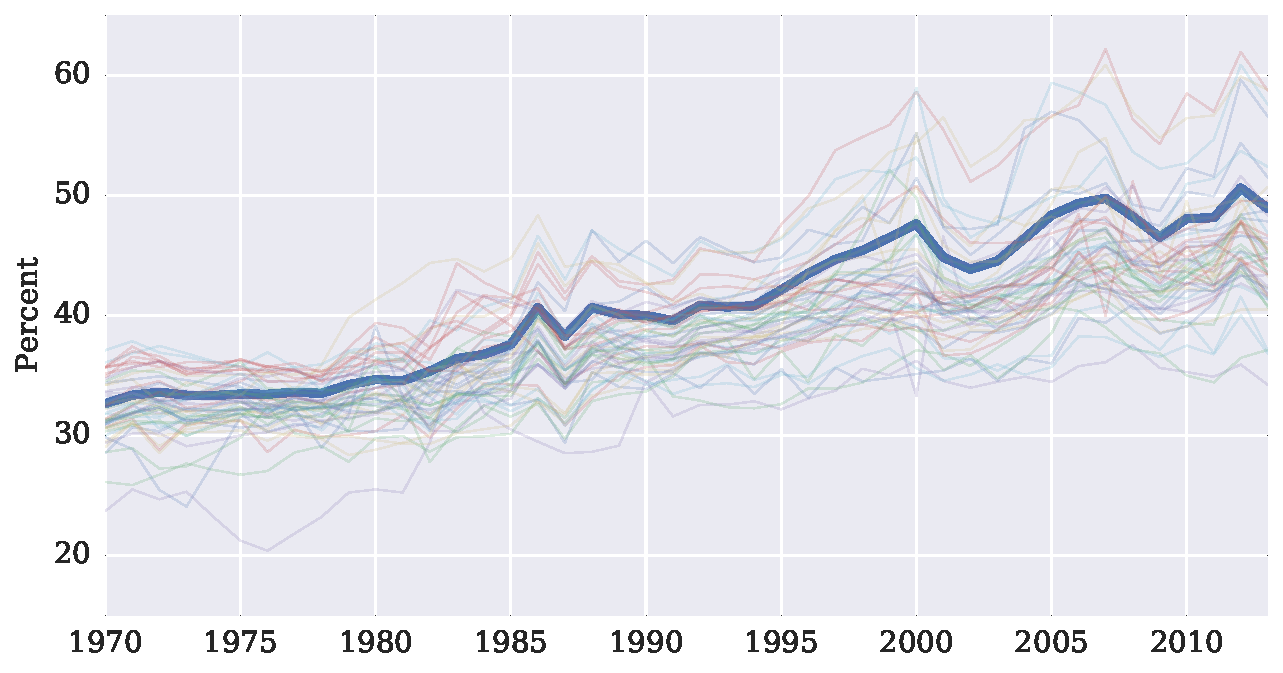
\includegraphics[width=6.3in]{../figures/inc_inequality/UnitedStates_Inc10_timeline.pdf}
	\end{center}
	\end{figure}


	\item {\bf Income Shares: Top 1\%}\\
	 Figure~\ref{fig:P1_US_timeline} depicts the income share for the top 1\% of income earners, which is similar in most respects to the top 10\% income shares. The US trend increases from about 9\% in 1970 to about 20\% in 2013, with decreases during recessions. The distribution of income shares across individual states varies more dramatically for this measure that the top decile income shares. In 2013, the lowest income share is around 11\% while the highest 1\% income share is nearly 3 times larger at about 31\%. As with the 10\% income shares, the trend for all states is both increasing and increasingly varied over time.

	\begin{figure}[htb!]  	
	\begin{center}	
	\caption{US Top 1\% Income Share (1970-2013) \label{fig:P1_US_timeline}}	
	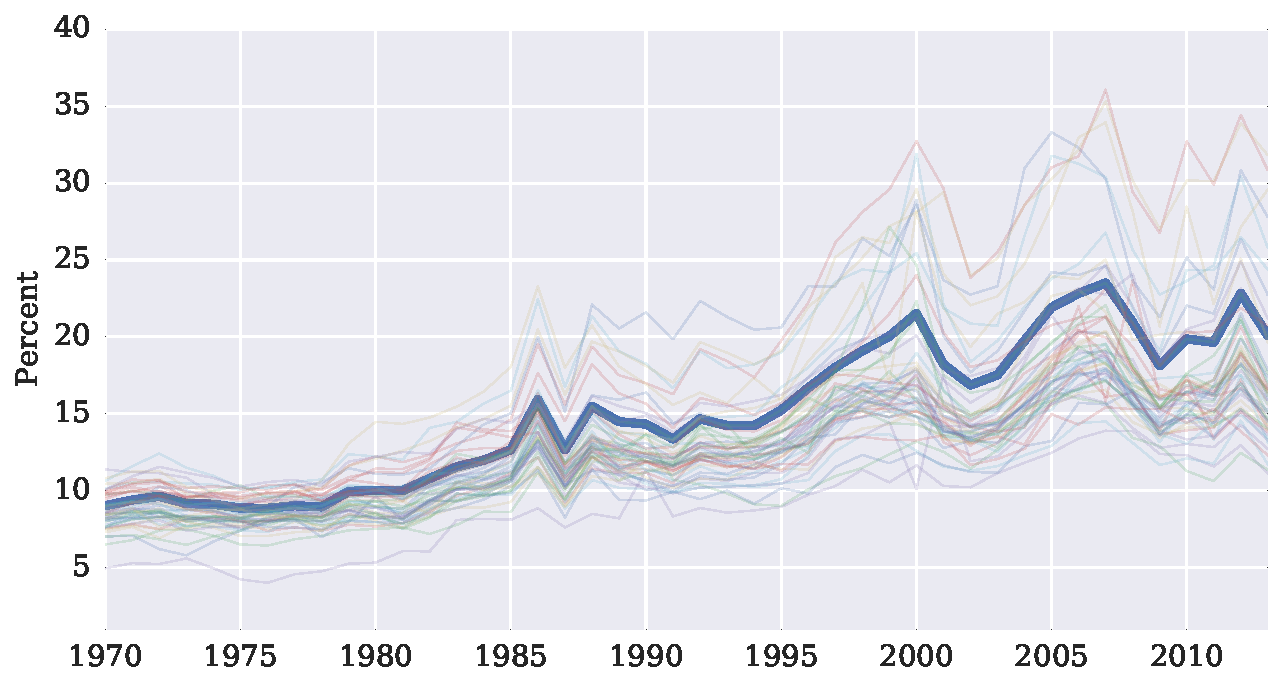
\includegraphics[width=6.3in]{../figures/inc_inequality/UnitedStates_Inc1_timeline.pdf}
	\end{center}
	\end{figure}		


	\item {\bf Gini Coefficients}\\
	I additionally use Gini coefficients as a measure of income inequality. The Gini coefficient is bounded to the [0,1] interval, in which an index of 0 occurs when all individuals have the same income and an index near 1 indicates a small number of individuals account for nearly all the income earned. As a measurement of inequality, Gini coefficients differ from income shares of top percentiles in that they account for the entire distribution of income. Consequently Gini coefficients will vary depending on how income is distributed above or below a given percentile, while the income share itself will remain the same. See \cite{frank2009inequality} for details on how this index is computed using IRS data. Figure~\ref{fig:gini_timeline} in Appendix A depicts the US Gini coefficient over time. Much like the income shares in Figure~\ref{fig:P10_US_timeline}, the US Gini coefficient is increasing while individual states have become increasingly dispersed around the national trend. The most notable difference is that the income shares in Figures~\ref{fig:P10_US_timeline} and ~\ref{fig:P1_US_timeline} vary visibly with the business cycle whereas the Gini coefficient is more stable. 

	\begin{figure}[htb!]  	
	\begin{center}	
	\caption{US Gini Coefficients (1970-2013) \label{fig:gini_timeline}}	
	\includegraphics[width=6.3in]{../figures/inc_inequality/UnitedStates_gini_timeline.pdf}
	\end{center}
	\end{figure}

\end{itemize}

The three measures are similar in many respects. The income share measures are strongly correlated with each other, with a contemporaneous correlation coefficient of .94. The Gini coefficient time series is highly correlated with both income share measures, with a correlation coefficient of .79 for both the top 10\% and 1\% income shares. Furthermore, the states with the highest and lowest values of inequality are generally common between the different measures (see online appendix for graphs of individual states).

\subsection{Geographic Patterns of Income Inequality}
An important pattern that arises at the state level is that income inequality often grows at similar rates among neighboring states. This suggests that regressions using state-level data for income inequality should cluster standard errors at a regional level of some kind. While there are many studies using the same state-level data as me, there are surprisingly few studies that cluster their standard errors and as a result are likely exaggerating the significance of their regression coefficients.

	\begin{figure}[htb!]  	
	\caption{Change in Top Decile Income Shares: 1970-1974 to 2009-2013 \label{fig:P10_map}}	
	This figure depicts the percent change in income inequality as measured by the top 10\% income share. The percent change is measured between the mean income share over 1970-1974 and the mean income share over 2009-2013.
	\begin{center}	
	\includegraphics[width=6.75in]{../figures/maps/Inc10_map.pdf}
	\end{center}
	\end{figure}

	\begin{figure}[htb!]  
	\caption{Change in Gini Coefficients: 1970-1974 to 2009-2013 \label{fig:gini_map}}	
	This figure depicts the percent change in income inequality as measured by Gini coefficients. The percent change is measured between the mean Gini coefficient over 1970-1974 and the mean Gini coefficient over 2009-2013.		
	\begin{center}
	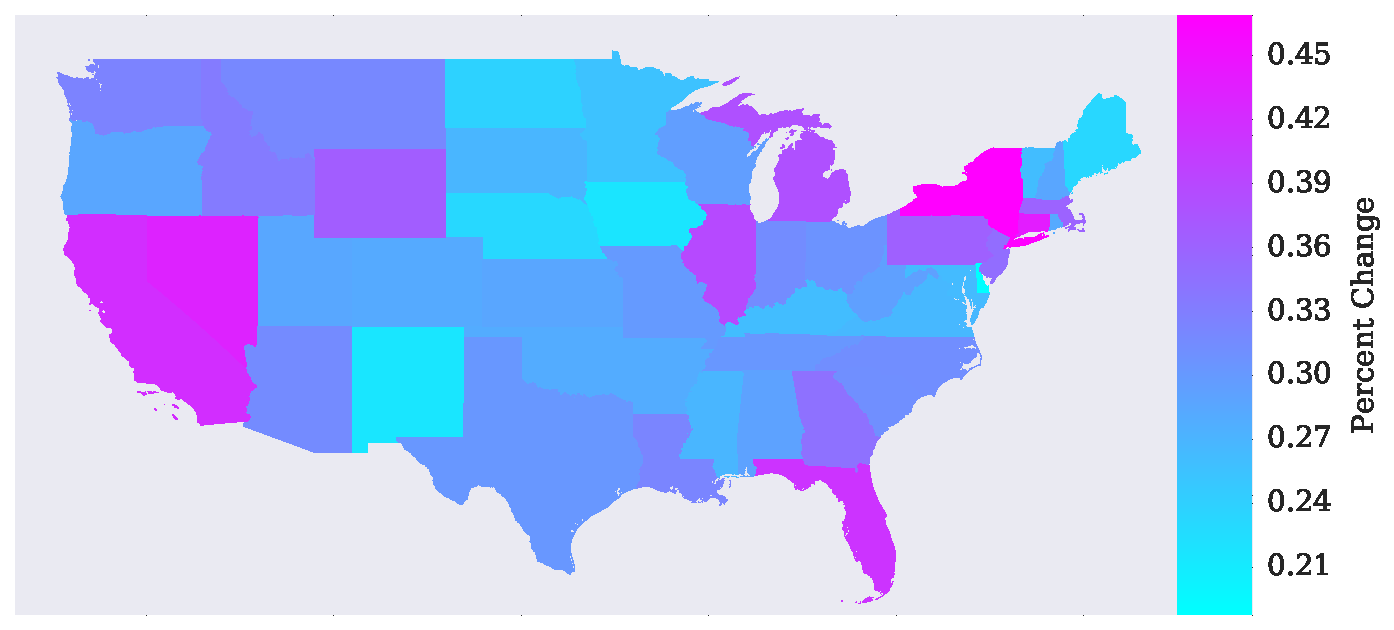
\includegraphics[width=6.75in]{../figures/maps/gini_map.pdf}
	\end{center}
	\end{figure}

Figure~\ref{fig:P10_map} shows the percentage change in income inequality over 1970-1974 and 2009-2013, as measured by the top decile income share. Figure~\ref{fig:gini_map} similarly depicts the percentage change in 5-year averages for Gini coefficients in each state over the same time interval. The maps are similar in that they both demonstrate geographic clustering for states with large increases in inequality. In both maps, States with large increases in inequality are most notably clustered in the Northeast around New York and in the Southwest around Nevada/California. The states with the three largest increases in top decile income shares over this time frame are Nevada (77\%), Connecticut (73\%), and New York (64\%). As measured by increases in Gini coefficients, the top three states are New York (47\%), Connecticut (44\%), and Nevada (43\%).

The similarities between the maps are less striking when it comes to areas where income inequality has grown at slower rates. In the map for income shares (Figure~\ref{fig:P10_map}), states with smaller gains in inequality are clustered in three regions: the Central Plains around Nebraska, the Deep South near Louisiana, and the Virginia/Maryland region. In the map based on Gini coefficients (Figure~\ref{fig:gini_map}), the Nebraska/Iowa region still stands out as an area with particularly low growth in income inequality. The Louisianna/Mississippi and Virginia/Maryland regions, however, demonstrate more moderate gains in inequality. As measured by the top 10\% income share, the states with the three lowest increases are Nebraska (21\%), Iowa (23\%), and Mississippi (24\%). As measured by increases in Gini coefficients, the bottom three states are Delaware (19\%), Hawaii (not shown, 21\%), and New Mexico (21\%). 


\subsection{Control Variables}
My goal is to measure, as much as possible, the relative contribution of several possible causes to the increase in income inequality over the past 30+ years. To do this I combine data from a variety of sources to control for, as much as possible, each of these trends simultaneously. These data are listed in Table~\ref{tab_indep_var}. Additional details, including sources, are listed in Table~\ref{ApdxTab_data_description}.

\begin{table}[htb!]
\caption{Independent Variables: potential causes of income inequality} \label{tab_indep_var}
\centering
\begin{tabular}{l|l|c}
 \hline  
 \hline	
	{\bf Potential Cause} & {\bf Variable(s)} & {\bf Availability} \\ 
	&&\\ \hline 
	&&\\
	\multirow{1}{*}{Skill-Biased  }			& - Patents counts   & 1970-2013 \\
	\multirow{1}{*}{Technological Change  }	& - IT share of GDP 		&  1997-2013\\ 
											& - Share of population with high school diploma  	& 	1970-2013 \\
	 										& - Share of population with college degree (4 year or equivalent) 		&  	1970-2013\\  
	&&\\ \hline 
	&&\\
	\multirow{1}{*}{Globalization } & - Total international exports (\% of state GDP) &  1999-2013\\ 
	&&\\ \hline 
	&&\\
	\multirow{1}{*}{Taxes }	& - Maximum marginal income tax rates   							& 1977-2013 \\
							& - Average marginal income tax rates (1984 income dist.)   & 1977-2013 \\
	&&\\ \hline 
	&&\\
	\multirow{1}{*}{Demographics }  & - Percent retired (age 65+)  								&  	1970-2013 \\
	 								& - Dependancy ratio  	& 	1970-2013 \\
	 								& - Percent racial/ethnic minority  						&  	1970-2013 \\
	&&\\ \hline 	
	&&\\ 
	\multirow{1}{*}{Finance Boom } 	& - Finance, insurance, \& real estate share of employment	& 1970-2013 \\
									& - Finance, insurance, \& real estate share of GDP			& 1987-2013 \\
	&&\\ \hline 
	&&\\
	\multirow{1}{*}{Entrepreneurship }	& - Startup density (age 0 firms per 100k people) &  1977-2013 \\
	 									& - Startup rate  										& 1977-2013 \\
	&&\\ \hline 		
\end{tabular}
\end{table}


I use a number of measures to capture the rate and location of skill-biased technological change, including education rates, the Information sector's share of GDP, and the number of patents originating within a given state each year. Education rates are a common, though crude, approximation for skill (see \cite{heckman1998explaining} for relevant examples). My data include the fraction of the population with high school and college level education as compiled in \cite{frank2009inequality}. These education levels vary considerably over time and across states. In 1980, the states with the lowest fractions of college attainment are West Virginia, Arkansas, and Kentucky at 6.7\%, 6.8\%, and 6.9\% respectively. In the same year, the states with the highest levels of college attainment are Colorado, Connecticut, and Massachusetts at 14.3\%, 13.7\%, and 13.4\% respectively. College attainment levels increase gradually over time for all states. In 2013 the lowest three states in terms of college attainment are Wyoming, Arkansas, and Mississippi at 14.5\%, 14.6\% and 15.1\% (a little better than the highest states in 1980), while the highest three states are Massachusetts, Maryland, and New Hampshire at 30.2\%, 29.3\% and 28.9\% respectively. Contiguous data on the Information sector's share of GDP is only available starting in 1997, and is available from the Bureau of Economic Analysis (BEA). 


My measure of globalization is the value of goods exported by states to foreign countries, measured as a percentage of GDP. Historical data on international trade at the State level are only available starting in 1999.\footnote{The census has only recently started to collect these data.} The data are depicted by state in the Appendix. For most states, exports as a share of GDP is either stationary or slightly increasing between 1999 and 2013. Although some states demonstrate increases in exports/GDP, it is difficult to determine whether the time series is stationary when the available time frame is so short.  States with large increases in exports as a percentage of GDP include Alabama, Idaho, Illinois, Kentucky, Louisiana, Mississippi, Nevada, North Dakota, South Carolina, Tennessee, Texas, Utah, Washington, and West Virginia. Due to the lack of data, I only use this measure in some regressions. 


I use two tax measures to control for the affect of tax rates on income inequality, both from \cite{feenberg1993taxsim} with updates provided by the NBER. The data are depicted by state in the Appendix. The first is the maximum marginal income tax rate, which is relevant as increases in income inequality in recent decades are driven by increasing wages among high income earners. An alternative measure is the average marginal income tax rate, which is estimated via simulation while holding the distribution of income fixed at 1984 levels. Holding the distribution of income fixed is important in overcoming an obvious endogeneity problem between average marginal tax rates and the distribution of income. Maximum tax rates vary considerably across states. In 2013, California and Hawaii have the highest income tax rates at 14.1\% and 11\% respectively. States with no income tax include Alaska, Florida, Nevada, New Hampshire, South Dakota, Tennessee, Texas, Washington, and Wyoming. For most states, rates vary occasionally over time and by small amounts. There are rare episodes of major tax changes, including Alaska decreasing its maximum tax rate from 14.5\% to 0\% in 1979, and Virginia increasing its maximum rate from 0\% to 5.82\% in 1991. Average tax rates demonstrate similar dynamics. For this measure I use the sum of Federal and state taxes since the data is more complete.\footnote{The state only table on the NBER website series is missing data for 2009. Since Federal rates are the same across all states, using total taxes should not affect my results in any meaningful way. }


To control for several concurrent demographic trends, I use the percent of population aged 65 or older as a proxy for the retired portion of the population. I also use the ``dependency ratio,'' which is determined by dividing the population of retirees and children (age 15 and younger) by the working age population (ages 16-64). I additionally control for black and minority populations, measured as a percentage of total population for each state. The retired percent of the population, depicted in Appendix [TODO] is gradually increasing in all states between 1970 and 2013. While there is some variance across states, the variance does not appear to increase over time. In spite of a generally increasing share of the retirees, the general trend for the dependency ratio is increasing only until around 1990's, after which the dependency ratio is on a clear downward trend until around 2005.


According to \cite{bakija2012jobs}, financial professionals comprise an increasingly large share of top income earners.\footnote{Between 1979 and 2005, the share of financial professionals among the top .1\% of income earners grew from 11\% to 18\%. They suggest a combination of corporate governance, the stock-market, and entrepreneurship may explaining much of the rise in top income shares.}  I use data on output and employment for the Finance, Insurance and Real Estate sector (FIRE). These variables are respectively measured as percentages of total GDP and employment, and both are provided by the BEA as depicted in Appendix [NUMBER]. Unfortunately, state-level data is only available starting in 1987, but there is only evidence for sustained growth in FIRE as a share of GDP after 1995 in most states. In 2013, the states with the highest share of GDP contributed by FIRE include Delaware, New York, and Connecticut at 40.0\%, 30.2\%, and 27.3\% respectively. The lowest states include Alaska, West Virginia, and Oklahoma at 10.7\%, 12.7\% and 13.3\% respectively. Growth in the output share of FIRE is depicted geographically in Figure [NUMBER HERE], with growth rates determined by comparing the 5 year average FIRE/GDP ratios for 1987-1991 and 2009-2013. States demonstrating exceptionally rapid growth in the FIRE share of GDP include Delaware and South Carolina, with percentage growth of 112.74\% and 116.75\%, respectively. Interestingly, the increase in the output share of FIRE is not concurrent with an increase in the employment share of FIRE. While the fraction of employment in the FIRE sector varies considerably across states, there is no notable growth over time in employment shares, even for states with rapidly growing GDP shares like Delaware and South Carolina.


I measure entrepreneurship rates using the number of new firms (age 0) per 100-thousand people. This data are compiled by the Kauffman Foundation at the state level using data the Bureau of Labor Statistics (BLS). Entrepreneurship has been decreasing steadily decreasing in the US since the late 1970's, as documented in \cite{decker2013secular,decker2014role,karahan2015understanding}. This trend is concurrent with the increase in income inequality. \cite{bakija2012jobs} examines the job types of upper income earners and states that entrepreneurship, in conjunction with other changes, is a likely candidate for explaining much of the most recent increases in income inequality. As depicted in Appendix [XYZ], all states demonstrate declining entrepreneurship rates between 1977 and 2013. I measure growth by comparing the change in levels for entrepreneurship rates between five-year averages over 1977-1981 and 2009-2013. The states with the largest declines are Nevada, Alaska, and Wyoming, with 182.8, 181.5, and 174.6 fewer age-zero firms per 100 thousand people, respectively.\footnote{I use changes in levels rather than percentage changes as the percentage changes seem to exaggerate changes for states with small populations.} The smallest declines are New York, Illinois, and Pennsylvania with 17.5, 49.2, and 50.9 fewer age-zero firms per 100 thousand people. 




\subsection{Econometric Analysis}

\subsubsection{What are the long-run drivers of income inequality?}
There are a number of issues within the data which I must address in order to appropriately estimate the relationship between income inequality and the various explanatory variables.  First, many of these variables are non-stationary, including measures of inequality, education, entrepreneurship, patent counts, and GDP shares for Information and FIRE sectors. To address this, I use an approach with accounts for the possibility of cointegration.  Second, growth in income inequality varies substantially across states and regions. Since I have a sufficiently long time series for each state, I could estimate the relationship for each state individually. This is not ideal, however, as the time-series for a single state is limited to less than 40 observations per state, and individual state regressions would ignore trends common across states. Still, a standard Fixed Effects (FE) estimator which requires slope coefficients to be constant across states may yield biased results considering the difference in income-inequality growth across regions. To overcome this problem, I use two techniques proposed in \cite{pesaran1997pooled,pesaran1999pooled} which allow for some heterogeneity in coefficients across panels without ignoring the long-term trend common across states. The first of these techniques, the mean-group (MG) estimator, simply averages the coefficients across single-panel regressions. The second technique, the pooled mean-group (PMG) estimator, pools coefficients for long-term trends while averaging single-panel coefficients for short-term phenomena. As a benchmark, I also use a standard Fixed-Effect estimator with standard errors clustered at the regional level.

\subsubsection{MG and PMG estimators}
I provide a concise description of the MG and PMG panel estimators as derived in \cite{pesaran1997pooled,pesaran1999pooled}.\footnote{For details on implementation, I recommend \cite{blackburne2007estimation}. } Assume the general panel specification 
\begin{eqnarray}\label{eq:mg_est_setup}
y_{it} = \sum_{j=1}^n \gamma_{ij} y_{i,t-j} + \sum_{j=0}^m \beta_{ij}' X_{i,t-j} + \alpha_i +\varepsilon_{it}
\end{eqnarray}

In my setting, $y_{it}$ is a measure of income inequality (income shares or gini coefficients), with states indexed by $i$ and time indexed by $t$. The variable $\alpha_{i}$ is the state-specific intercept, $X_{i,t-j}$ is a vector of control variables with coefficient vector $\beta{ij}$, and $\varepsilon_{it}$ is a state-specific error term. Many of my variables are nonstationary and cointegrated, and thus are sensitive to short-term deviations from long-run trends. Consequently I estimate an error-corrected version of \eqref{eq:mg_est_setup} which includes a short-term ``error-correction'' term separate from the long-term trend
\begin{eqnarray}\label{eq:mg_est}
\Delta y_{it} = \phi_{i}\left(y_{i,t-1} - \theta_i'X_{i,t} \right) +\sum_{j=1}^{n-1} \gamma^*_{ij} \Delta y_{i,t-j}+ \sum_{j=0}^{m-1} \beta^{*'}_{ij} \Delta X_{i,t-j} + \alpha_i +\varepsilon_{it}.
\end{eqnarray}
Here $\phi_{i} = -\left(  1-\sum_{j=1}^p \gamma_{ij} \right)$ is the speed of error-adjustment and should be significantly negative if variables regularly return to their long-run trend. The variable $\theta_i = \sum_{j=0}^q \beta_{ij}/\left(1-\sum_k\lambda_{ik}\right)$ gives the long run relationship between the independent and dependent variables. Other variables
$\lambda^*_{ij} = -\sum_{m=j+1}^p \lambda_{im}$ for $j=1,\mathellipsis, p-1$, and $\delta^*_{ij}=-\sum^q_{m=j+1}\delta_{im}$ for $j=1,\mathellipsis, q-1$ are similar to their counterparts in \eqref{eq:mg_est_setup}.

The PMG technique estimates the parameters in \eqref{eq:mg_est} using maximum likelihood \citep{pesaran1999pooled}. The MG method simply averages regression coefficients over the individual panels. Table~\ref{tab:regressions} gives the estimation results for the MG and PMG estimates, along with standard FE estimates. 



\subsection{Results}

\begin{footnotesize}
\begin{table}[htb!]
\centering
\caption{Current}\label{tab:regressions}
\begin{tabular}{l|lccc} \hline 
& Variable & MG & PMG & DFE \\ \hline 
\parbox[t]{2mm}{\multirow{12}{*}{\rotatebox[origin=c]{90}{Short Run}}} & & & \\ 
&$\hat{\phi}$&   -0.839*** &   -0.438*** &   -0.335*** \\
& &   (0.0318) &   (0.0280) &   (0.0310) \\
&$\Delta$WageTax\_total &   -0.0335*** &   -0.0471*** &   -0.0399*** \\
& &   (0.0130) &   (0.0112) &   (0.0108) \\
&$\Delta$ent1 &   0.00687 &   0.0578*** &   0.0613*** \\
& &   (0.0146) &   (0.0111) &   (0.00872) \\
&$\Delta$pct\_black &   -0.0204 &   -0.0610 &   0.0781 \\
& &   (0.256) &   (0.249) &   (0.0877) \\
&$\Delta$pct\_retired &   -1.545*** &   -0.684*** &   -0.455*** \\
& &   (0.208) &   (0.119) &   (0.150) \\
&$\Delta$patents\_percapita &   0.00913 &   0.0128 &   -0.00942 \\
& &   (0.00703) &   (0.00840) &   (0.00774) \\
&$\Delta$College &   -0.0796*** &   -0.0601*** &   -0.0366* \\
& &   (0.0241) &   (0.0212) &   (0.0217) \\
&$\Delta$fire\_pct &   -0.0451 &   0.0275 &   0.00313 \\
& &   (0.0519) &   (0.0357) &   (0.0321) \\
&  &  &  &  \\ \hline 
\parbox[t]{2mm}{\multirow{12}{*}{\rotatebox[origin=c]{90}{Long Run}}} & & & \\ 
&WageTax\_total & -0.0132   & 0.0207   & -0.0141   \\
& & (0.0198)   & (0.0130)   & (0.0207)   \\
&ent1 & 0.0764***   & -0.00611   & -0.0287   \\
& & (0.0215)   & (0.0163)   & (0.0336)   \\
&pct\_black & 0.563***   & 0.0292**   & -0.0117   \\
& & (0.172)   & (0.0127)   & (0.0240)   \\
&pct\_retired & 0.414***   & 0.196***   & 0.177**   \\
& & (0.111)   & (0.0307)   & (0.0808)   \\
&patents\_percapita & 0.00119   & 0.0146*   & 0.0390***   \\
& & (0.0171)   & (0.00772)   & (0.0124)   \\
&College & 0.159***   & 0.245***   & 0.237***   \\
& & (0.0473)   & (0.0195)   & (0.0389)   \\
&fire\_pct & 0.112*   & 0.106***   & 0.101**   \\
& & (0.0627)   & (0.0286)   & (0.0431)   \\
&&&&\\ \hline 

& Observations & 1,750 & 1,750 & 1,750 \\ 

& Num. groups  & 50 & 50 & 50 \\ 

& Obs. per group  &35&35&35\\ 
\end{tabular} 

\end{table}
\end{footnotesize}




\subsubsection{Have the drivers of income inequality changed over time?}
An inherent assumption within the previous regression results is that the causes of income inequality have remained constant over the observed time-frame. This notion is also absent in any regression analysis that lacks time-varying elements, which is true for the vast majority of empirical work in the income inequality literature (citations here). 

To identify movements over time in the relative importance of any particular variable in explaining income inequality, I run a simple cross-sectional regression for each year in the panel (1977-2013) and compare the coefficients over time. Figure X displays these coefficients for each year, with stars denoting statistically significant coefficients at the .95\% level. 

INSERT FIGURES HERE.




\section{Model}
Time is discrete and indexed by $t = 1,2,\mathellipsis$. The economy is comprised of a continuum of finitely lived families or households. Households live for $N$ periods, with age indexed by $h_1, \mathellipsis, h_N$. The measure of households at age $h_i$ in period $t$ is given $\mu_t(h_i)$. Newly born households live through 3 phases of life: human capital accumulation, working, and retirement. Human capital accumulation takes place in a single period, while the working and retirement phases last for several periods. Households die with certainty at age $h_N$.

\subsection{Human Capital Investment}
A newly born household realizes bequests $a_0$ and productivity $z_0$, and chooses an amount to invest in human capital $hc\in[0,1]$. Bequests $a_0\geq 0$ are drawn from a distribution determined by the assets of dying households. Only a share $\gamma\in[0,1]$ of dying households will choose to bequest their remaining wealth in their final period of life. Consequently, only some new households will receive nonzero bequests. Productivity $z_0$ is drawn from a distribution $G(z)$. This initial productivity draw serves only to guide the expectations of future productivity levels and in turn the household's human capital investment decision. The cost of the human capital investment $d$ is drawn from a distribution $G(d)$ after the human capital investment is made.

Mathematically, a household in this phase solves the following maximization problem:
\begin{eqnarray}
&&\hat{V}_{h_0}(a_0,z_0,k_0)=\max_{hc} E_t\left[ \hat{V}^w_{h_1}(a_1,z_1,0)\right] \\
\text{subject to} 	&& a_1 = a_0 - d, \;\; d = hc^\alpha, \\
					&& z_1 = \rho_z z_0 + \sigma_z\epsilon_t + hc, \;\; \epsilon_t\sim N(0,1).
\end{eqnarray}
Here $V_0$ is the lifetime utility of a household at age $h_0$. The value $E_t\left[ \hat{V}^w_{h_n}(a_1,z_1,k_1)\right]$ gives the expected lifetime utility of the household at the start of the working phase after making a human capital investment of $hc$. The variable $a_1$ is the difference between the household's initial wealth and the debt incurred through its human capital investment. Households in this phase cannot hold or acquire business capital. Hence business capital at birth $k_0$ and after human capital investment are both equal to zero. Finally, $\rho_z$ and $\sigma_z$ govern the persistence and volatility of productivity.


\subsection{Working and Production}
Households in the working phase observe their previous productivity level $z_{t-1}$ and wealth $a_t$. The households then choose to work for a firm or to start their own business. Households who choose to work for a firm will inelastically contribute a unit of labor in exchange for a wage which can used for consumption $c_t$ or to augment their wealth. In the spirit of \cite{hopenhayn1993job}, households to choose to start a firm pay an entry cost $c_f$. After entering, firms invest in capital, produce, and earn profits. Profits are retained by firm owners to finance their personal consumption and savings. Firms realize their new productivity $z_1$ after deciding whether or not to start a firm. 

After paying their entry cost, new firms observe their productivity and draw an initial stock of capital $k_t$ from a distribution $G(k)$. Incumbent firms simply observe their existing stock of capital. Firms then choose capital investment $i_t$, pay wages and operating expenses, and make their individual consumption and savings decision. Labor supply, $n_t$, is the same for all firms and evenly allocates working households across firms.\footnote{ In comparison to \cite{hopenhayn1993job}, I have simply traded a rich firm-size distribution and degenerate wage for a rich wage distribution and single firm-size. By introducing capital, something absent from \cite{hopenhayn1993job}, I can still maintain a sense of firm size and some control over entry/exit flows.
} 
Each period, firm owners face additional expenses of wages, a capital adjustment cost $\Phi(i_t,k_t)$, and a fixed operating cost $c_j$ to be paid each period while the firm is in operation. Remaining profits are then used for consumption and personal savings. If at the start of a period a household-owning firm expects profits to be negative for some time (say, due to the persistent nature of productivity), it may exit firm ownership and instead work for an existing firm. 


\subsubsection{Entry and Exit}
The entry/exit decision is made at the start of the period, before productivity $z_t$ is realized. If a firm-owner exits, the household parts with its existing business capital which is discarded at no cost or benefit. The firm-owner still must pay a capital adjustment cost of $\Phi(i_t,k_t)$. Exiting firm-owners, however, do not pay the per-period expense $c_j$, and may instead earn a wage as an employee within the period. Mathematically, the entry/exit decision for an incumbent firm-owner is given by:
%
\begin{eqnarray}\label{}
\hat{V}^f_{h_n}(a_t,z_{t-1},k_t)=\max\left\{ E_t\left[ V^w_{h_n}(a_t,z_t,0)-\Phi(0,k_t) \right],\; E_t\left[ V^f_{h_n}(a_t,z_t,k_t)\right]\right\}.
\end{eqnarray}
%
Here $\hat{V}^f_{h_n}(a_t,z_{t-1},k_t)$ is the lifetime utility of an incumbent firm-owner at the time of its exit decision. The value $E_t\left[ V^w_{h_n}(a_t,z_t,0)-\Phi(0,k_t) \right]$ corresponds to the expected lifetime utility of the household if it exits firm-ownership. The term $E_t\left[ V^f_{h_n}(a_t,z_t,k_t,n_{t-1})\right]$, corresponds to the expected lifetime value from continuing as a firm owner. 

The maximization problem for a working household is similarly given by:
\begin{eqnarray}
&& \hat{V}^w_{h_n}(a_t,z_{t-1},0)=\max\left\{ E_t\left[ V^w_{h_n}(a_t,z_t,0) \right],\; E_t\left[ V^f_{h_n}(a_t,z_t,k_t)-c_f\right]\right\} 
\end{eqnarray}
Here $\hat{V}^w_{h_n}(a_t,z_{t-1},0)$ is the lifetime utility of a working household at the time of its entry decision. A household will choose to start a firm if the expected payoff from doing so, net of entry cost $c_f$, is greater than the expected payoff from continuing to work as an employee. Capital is equal to zero since working households cannot hold business capital. In both cases, expectations are taken over future productivity levels which evolve according to an AR(1) process
\begin{eqnarray}
z_{t+1} = \rho_z z_t + \sigma_z\epsilon_{t+1}; \;\; \epsilon_t\sim N(0,1). 
\end{eqnarray}


\subsubsection{Matching and Production}
Working households are evenly divided among firm-owners. While clearly unrealistic, this simplifying assumption allows me to pair heterogeneous workers and firms of various quantities without violating market clearing. 

I consider two methods of assigning workers to firms. The first method, randomly assigns an equal number of workers to each firm. The second method ranks $N$ workers and $M$ firms by productivity, then assortatively matches $M$ subsets of workers to the $M$ firms according to their rank. In this way, the most productive $N/M$ workers match with the most productive firm, the next-most productive $N/M$ workers match with the next-most productive firm, and so on. 

 A firm may match with several workers, who produce independently of each other.\footnote{This arrangement is important in generating a rich wage distribution. If only aggregate labor (i.e. the sum of productivities) appeared in the production function, all workers would have the same marginal productivity. CES aggregators, while allowing for different marginal productivities, are computationally infeasible for a continuum of heterogeneous workers.} The total output of the firm is simply the sum of individual outputs from each worker. The output of a worker-firm pair worker depends on their respective productivities ($z_i$, $z_j$), as well as the firm's capital per worker $\bar k_t = k_t/n_t$:
\begin{eqnarray}\label{eq:production_decentralized}
y_i = z_j z_i^{1-\alpha} \bar k^\alpha, \;\; \alpha\in(0,1).
\end{eqnarray}
The working household's wage is equal to its marginal productivity
\begin{eqnarray}
w_i= (1-\alpha)z_j\left( \frac{\bar k}{z_i} \right)^{\alpha}.
\end{eqnarray}
Within a firm, marginal productivities (and therefore wages) will differ between workers based on their productivity levels. Marginal productivities, however, will still be correlated at the firm-level through the common inputs contributed by the firm owner. This will allow me to compare my model through the lens of \cite{song2015firming}, who show most income inequality growth since the late 1970's has occurred across firms rather than within firms.


Let $J$ be the distribution of worker productivities employed by firm owner $j$. Total output $Y_j$ is simply the sum/integral of the individual outputs of households working for firm $j$:
\begin{eqnarray}
Y_j = \int y_i \diff J.
\end{eqnarray}
%
For a firm with capital stock $k_t$ and investment $i_t$, profits are given by total output net of wages, adjustment cost $\Phi(i_t, k_t)$, and the per-period operating cost $c_j$: 
\begin{eqnarray}
\Pi_j(i_t, k_t) =  \int \left( y_i - w_i \right) \diff J - \Phi(i_t, k_t) - c_j.  
\end{eqnarray}


Once production occurs and wages and profits are realized, and all households make their optimal consumption/savings decision. These optimization problems are given respectively for working and firm-owning households of ages $h_n<h_{R-1}$:
\begin{eqnarray}
&& V^w_{h_n}(a_t,z_t,0) = \max_{c_t,a_{t+1}} u(c_t) + \beta E_t\left[ \hat{V}^w_{h_{n+1}}(a_{t+1},z_{t},0) \right] \label{eq:V_working} \\
\text{subject to } && c_t + a_{t+1} \leq w_t + r_t a_t. \label{eq:budget_constraint_working} \\
				   && \notag\\ 
&& V^f_{h_n}(a_t,z_t,k_t) = \max_{c_t,a_{t+1},i_t} u(c_t) + \beta E_t\left[ \hat{V}^f_{h_{n+1}}(a_{t+1},z_{t},k_{t+1}) \right] \label{eq:V_firmowning} \\
\text{subject to } && c_t + a_{t+1} \leq \Pi_t(i_t,k_t) + r_t a_t, \label{eq:budget_constraint_firmowning} \\
				   && k_{t+1} = k_t(1-\delta) + i_t \label{eq:capital_law_of_motion}
\end{eqnarray}
Here, $V^w_{h_n}(a_t,z_t,0)$ is the expected lifetime utility for a working household of age $h_n$. Equation~\eqref{eq:budget_constraint_working} is the working household's budget constraint, in which liquid assets $a_t$ are riskless and accumulate interest at rate $r_t$. The value $V^f_{h_n}(a_t,z_t,k_t)$ is the expected lifetime utility of a firm-owning household. Equation~\eqref{eq:budget_constraint_firmowning} is the firm-owning household's budget constraint. Equation~\eqref{eq:capital_law_of_motion} is the law of motion for capital accumulation with constant depreciation rate $\delta$.

If a household is of age $h_n=h_{R-1}$, its optimization problem changes slightly since the household is obligated to retire the following period. Consequently, the expectation terms in  \eqref{eq:V_working} and \eqref{eq:V_firmowning} are replaced with a common function $V^R_{h_R}(a_{t+1},z_t,0)$. The value of $V^R_{h_R}(a_{t+1},z_t,0)$ is equal to the expected lifetime utility of a retired household of age $h_R$ with wealth $a_{t+1}$. 


\subsection{Retirement}
Mandatory retirement occurs at age $h_R$. Upon retirement, firm-owners bequest a fraction $\gamma_K$ of their capital to households graduating from school. Retired households receive no income and consume out of their savings. A fraction $\gamma\in[0,1]$ of retired households leave a bequest to newly born households. Whether or not a household will leave a bequest is determined at random in the final period of life. The lifetime utility of a household in the final period of life with no bequest motive is given by:
%
\begin{eqnarray}
&& V_{h_N}(a_t) = \max_{c_t} u(c_t)\\
\text{subject to } && c_t = a_t
\end{eqnarray}
Here I ignore the state variables $(z_t,k_t)$ since they have no affect on retired households. If the household is selected to make a bequest $a_0$, an event that occurs with probability $\gamma$, their final maximization problem is given by 
\begin{eqnarray}
&& V^b_{h_N}(a_t) = \max_{c_t,a_0} u(c_t) + \nu(a_0)\\
\text{subject to } && c_t + a_0 = a_t.
\end{eqnarray}
%
Here $\nu(a_0)$ is a ``warm glow'' utility from leaving a bequest, with $\nu'(a_0)>0$ and $\nu''(a_0)<0$. The random nature of the bequest motive will affect the optimization problem leading up to age $h_N$. Specifically, the optimization problem at age $h_{N-1}$ is given by
\begin{eqnarray}
&& V_{h_{N-1}}(a_t) = \max_{c_t, a_{t+1}} u(c_t) + \beta \left[ (1-\gamma)V_{h_N} + \gamma V^b_{h_N} \right]\\
\text{subject to } &&  c_t +a_{t+1} = r_ta_t
\end{eqnarray}

The value function for all other periods of retirement takes the following form:
\begin{eqnarray}
&& V_{h_{n}}(a_t) = \max_{c_t, a_{t+1}} u(c_t) + \beta E_t\left[ V_{h_{n+1}}(a_t)\right], \\
\text{subject to } && c_t +a_{t+1} = r_ta_t.
\end{eqnarray}






\newpage
% ------------------------------------------------------------------
% References
% ------------------------------------------------------------------
\bibliography{wealth}{}
\bibliographystyle{ecta}
% ------------------------------------------------------------------



%%%%%%%%%%%%%%%%%% APPENIX %%%%%%%%%%%%%%%%%%

\newpage\clearpage\appendix\onehalfspacing\renewcommand{\theequation}{A.\arabic{equation}} \setcounter{equation}{0} 
%%% Repayment to Creditors
\section{Additional Figures}

\begin{landscape}
\begin{table}
\caption{Description of Variables used in Panel Regressions}
\label{ApdxTab_data_description}
\centering
\begin{tabular}{l|l|c}
 \hline  
 \hline	
	{\bf Variable} & {\bf Definition} & {\bf Source} \\ 
	&&\\ \hline 
	&&\\
	{\bf Skill-biased Tech. Change }	&& \\
	- Education (High school)  	& Share of population with high school education & \multirow{2}{*}{\cite{frank2009inequality}; \href{http://www.shsu.edu/eco_mwf/inequality.html}{[link to data]}}\\
	- Education (College)  	& Share of population with college education &\\
	 - Patents for inventions			& Utility patent counts by state 	&   US Patent and Trademark Office; \href{http://www.uspto.gov/web/offices/ac/ido/oeip/taf/cst_utlh.htm}{[link to data]} \\ 
	 - IT share of GDP					& IT GDP/Total GDP	 				&  BEA Regional Tables (Real GDP) \\ 
	&&\\ \hline 
	&&\\
	{\bf Globalization}  &&\\
	- Total exports &   	Value of goods exported/Total GDP								& \href{http://tse.export.gov/tse/tsehome.aspx}{International Trade Association} \\
	&&\\ \hline 
	&&\\
	{\bf Taxes (state and federal)}  & & \\
	- Maximum income tax rate & Income tax rate for highest tax bracket  	& \multirow{2}{*}{\cite{feenberg1993taxsim}; \href{http://users.nber.org/~taxsim/}{[link to data]}} \\
	- Average income tax rate & Average marginal tax rate (1984 income distribution) 	& \\
	&&\\ \hline 
	&&\\
	{\bf Finance Boom}  &&\\
	- Share of employment in FIRE & FIRE employment/Total employment & BEA (Tables SA25,SA25N)\\
	&&\\ \hline 
	&&\\
	{\bf Demographics}   &&\\
	- Percent Retired  & Age $>65$ population/Total population & \multirow{3}{*}{\href{https://www.census.gov/popest/data/historical/index.html}{Census}, author's calculations } \\
	- Dependancy Ratio & [Age $>65$ and age $<15$ population]/Age 15-65 population&  \\
	- Percent Black & Black population/Total population &  \\
	% - Percent Minority & [Black and Other population]/Total population &  \\
	&&\\ \hline 	
	&&\\ 
	{\bf Entrepreneurship} 	&&\\
	- Startup density &  Number of age 0 firms per 100k people &   \multirow{2}{*}{ \href{http://www.kauffman.org/microsites/kauffman-index/about/archive/kauffman-index-of-entrepreneurial-activity-data-files}{Kauffman Foundation - State Components} } \\
	- Startup rate && \\
	&&\\ \hline 		
\end{tabular}
\end{table}
\end{landscape}



\section{Regression Results}

\begin{footnotesize}
\begin{table}[htb!]
\centering
\caption{Top 10\%: benchmark }
\begin{tabular}{l|lccc} \hline 
& Variable & MG & PMG & DFE \\ \hline 
\parbox[t]{2mm}{\multirow{12}{*}{\rotatebox[origin=c]{90}{Short Run}}} & & & \\ 
&$\hat{\phi}$&   -0.839*** &   -0.438*** &   -0.335*** \\
& &   (0.0318) &   (0.0280) &   (0.0310) \\
&$\Delta$WageTax\_total &   -0.0335*** &   -0.0471*** &   -0.0399*** \\
& &   (0.0130) &   (0.0112) &   (0.0108) \\
&$\Delta$ent1 &   0.00687 &   0.0578*** &   0.0613*** \\
& &   (0.0146) &   (0.0111) &   (0.00872) \\
&$\Delta$pct\_black &   -0.0204 &   -0.0610 &   0.0781 \\
& &   (0.256) &   (0.249) &   (0.0877) \\
&$\Delta$pct\_retired &   -1.545*** &   -0.684*** &   -0.455*** \\
& &   (0.208) &   (0.119) &   (0.150) \\
&$\Delta$patents\_percapita &   0.00913 &   0.0128 &   -0.00942 \\
& &   (0.00703) &   (0.00840) &   (0.00774) \\
&$\Delta$College &   -0.0796*** &   -0.0601*** &   -0.0366* \\
& &   (0.0241) &   (0.0212) &   (0.0217) \\
&$\Delta$fire\_pct &   -0.0451 &   0.0275 &   0.00313 \\
& &   (0.0519) &   (0.0357) &   (0.0321) \\
&  &  &  &  \\ \hline 
\parbox[t]{2mm}{\multirow{12}{*}{\rotatebox[origin=c]{90}{Long Run}}} & & & \\ 
&WageTax\_total & -0.0132   & 0.0207   & -0.0141   \\
& & (0.0198)   & (0.0130)   & (0.0207)   \\
&ent1 & 0.0764***   & -0.00611   & -0.0287   \\
& & (0.0215)   & (0.0163)   & (0.0336)   \\
&pct\_black & 0.563***   & 0.0292**   & -0.0117   \\
& & (0.172)   & (0.0127)   & (0.0240)   \\
&pct\_retired & 0.414***   & 0.196***   & 0.177**   \\
& & (0.111)   & (0.0307)   & (0.0808)   \\
&patents\_percapita & 0.00119   & 0.0146*   & 0.0390***   \\
& & (0.0171)   & (0.00772)   & (0.0124)   \\
&College & 0.159***   & 0.245***   & 0.237***   \\
& & (0.0473)   & (0.0195)   & (0.0389)   \\
&fire\_pct & 0.112*   & 0.106***   & 0.101**   \\
& & (0.0627)   & (0.0286)   & (0.0431)   \\
&&&&\\ \hline 

& Observations & 1,750 & 1,750 & 1,750 \\ 

& Num. groups  & 50 & 50 & 50 \\ 

& Obs. per group  &35&35&35\\ 
\end{tabular} 

\end{table}
\end{footnotesize}



\clearpage
\newpage
\begin{footnotesize}
\begin{table}[htb!]
\centering
\caption{Top 10\%: benchmark + dependency ratio }
\begin{tabular}{l|lccc} \hline 
& Variable & MG & PMG & DFE \\ \hline 
\parbox[t]{2mm}{\multirow{12}{*}{\rotatebox[origin=c]{90}{Short Run}}} & & & \\ 
&$\hat{\phi}$&   -1.211*** &   -0.608*** &   -0.416*** \\
& &   (0.0411) &   (0.0461) &   (0.0354) \\
&$\Delta$WageTax\_total &   0.0131 &   0.0107 &   0.0121 \\
& &   (0.0153) &   (0.0138) &   (0.0120) \\
&$\Delta$ent1 &   -0.0506*** &   0.0710*** &   0.0914*** \\
& &   (0.0181) &   (0.0164) &   (0.0227) \\
&$\Delta$pct\_black &   -0.133 &   -0.485** &   -0.0637 \\
& &   (0.413) &   (0.238) &   (0.0683) \\
&$\Delta$pct\_retired &   -0.200 &   0.141 &   -0.304 \\
& &   (0.353) &   (0.152) &   (0.191) \\
&$\Delta$patents\_percapita &   -0.0511*** &   -0.0217*** &   -0.0251*** \\
& &   (0.0143) &   (0.00787) &   (0.00775) \\
&$\Delta$College &   -0.134*** &   -0.105*** &   -0.0906*** \\
& &   (0.0359) &   (0.0242) &   (0.0251) \\
&$\Delta$fire\_pct &   0.0464 &   0.0961* &   0.0281 \\
& &   (0.0769) &   (0.0535) &   (0.0591) \\
&  &  &  &  \\ \hline 
\parbox[t]{2mm}{\multirow{12}{*}{\rotatebox[origin=c]{90}{Long Run}}} & & & \\ 
&WageTax\_total & 0.0301*   & 0.0443***   & 0.0191   \\
& & (0.0175)   & (0.0130)   & (0.0225)   \\
&ent1 & 0.167***   & 0.0763***   & 0.0410   \\
& & (0.0246)   & (0.0149)   & (0.0359)   \\
&pct\_black & 0.284   & 0.0335***   & 0.0118   \\
& & (0.185)   & (0.0129)   & (0.0290)   \\
&pct\_retired & 0.722***   & 0.413***   & 0.282***   \\
& & (0.132)   & (0.0368)   & (0.0915)   \\
&patents\_percapita & 0.0331**   & 0.0162**   & 0.0283*   \\
& & (0.0156)   & (0.00721)   & (0.0159)   \\
&College & 0.232***   & 0.290***   & 0.299***   \\
& & (0.0576)   & (0.0201)   & (0.0385)   \\
&fire\_pct & -0.0121   & 0.0526*   & 0.0859**   \\
& & (0.0750)   & (0.0275)   & (0.0415)   \\
&&&&\\ \hline 

& Observations & 1,750 & 1,750 & 1,750 \\ 

& Num. groups  & 50 & 50 & 50 \\ 

& Obs. per group  &35&35&35\\ 
\end{tabular} 

\end{table}
\end{footnotesize}



\clearpage
\newpage
\begin{footnotesize}
\begin{table}[htb!]
\centering
\caption{Top 10\%: benchmark + minorities }
\begin{tabular}{l|lccc} \hline 
& Variable & MG & PMG & DFE \\ \hline 
\parbox[t]{2mm}{\multirow{12}{*}{\rotatebox[origin=c]{90}{Short Run}}} & & & \\ 
&$\hat{\phi}$&   -0.0942*** &   -0.0685*** &   -0.0421*** \\
& &   (0.0227) &   (0.00932) &   (0.00811) \\
&$\Delta$WageTax\_total &   -0.0259*** &   -0.0515*** &   -0.0487*** \\
& &   (0.00764) &   (0.00597) &   (0.00439) \\
&$\Delta$ent1 &   0.00435 &   0.00625 &   0.0132 \\
& &   (0.0101) &   (0.00793) &   (0.00806) \\
&$\Delta$pct\_black &   -0.342* &   -0.0621 &   0.0327 \\
& &   (0.177) &   (0.109) &   (0.0292) \\
&$\Delta$pct\_retired &   0.492*** &   0.337*** &   0.228*** \\
& &   (0.161) &   (0.0518) &   (0.0468) \\
&$\Delta$patents\_percapita &   0.0155*** &   0.0158*** &   0.00949** \\
& &   (0.00440) &   (0.00421) &   (0.00399) \\
&$\Delta$College &   -0.0123 &   0.000135 &   0.00619 \\
& &   (0.0134) &   (0.00932) &   (0.00790) \\
&$\Delta$fire\_pct &   -0.0199 &   0.00192 &   0.0321*** \\
& &   (0.0226) &   (0.0171) &   (0.0123) \\
&  &  &  &  \\ \hline 
\parbox[t]{2mm}{\multirow{12}{*}{\rotatebox[origin=c]{90}{Long Run}}} & & & \\ 
&WageTax\_total & -0.274   & -0.277***   & -0.633***   \\
& & (0.222)   & (0.0450)   & (0.143)   \\
&ent1 & 0.348   & 0.617***   & 0.648***   \\
& & (0.216)   & (0.0769)   & (0.154)   \\
&pct\_black & 1.749   & 0.736***   & -0.0362   \\
& & (1.171)   & (0.120)   & (0.0529)   \\
&pct\_retired & 0.497   & 0.0248   & 0.0751   \\
& & (0.995)   & (0.122)   & (0.160)   \\
&patents\_percapita & 0.0108   & 0.0841***   & 0.0351   \\
& & (0.0857)   & (0.0202)   & (0.0440)   \\
&College & 0.457   & 0.222***   & 0.263***   \\
& & (0.364)   & (0.0463)   & (0.0903)   \\
&fire\_pct & 0.372   & 0.418***   & 0.349**   \\
& & (0.385)   & (0.0727)   & (0.154)   \\
&&&&\\ \hline 

& Observations & 1,750 & 1,750 & 1,750 \\ 

& Num. groups  & 50 & 50 & 50 \\ 

& Obs. per group  &35&35&35\\ 
\end{tabular} 

\end{table}
\end{footnotesize}



% \clearpage
% \newpage
% \begin{footnotesize}
% \begin{table}[htb!]
% \centering
% \caption{Top 10\%: benchmark + High School }
% \begin{tabular}{l|lccc} \hline 
& Variable & MG & PMG & DFE \\ \hline 
\parbox[t]{2mm}{\multirow{12}{*}{\rotatebox[origin=c]{90}{Short Run}}} & & & \\ 
&$\hat{\phi}$&   -0.882*** &   -0.428*** &   -0.294*** \\
& &   (0.0312) &   (0.0333) &   (0.0263) \\
&$\Delta$WageTax\_total &   0.0330** &   0.00902 &   0.0136 \\
& &   (0.0129) &   (0.0104) &   (0.00897) \\
&$\Delta$ent1 &   -0.0594*** &   0.0187 &   0.0445*** \\
& &   (0.0160) &   (0.0129) &   (0.0162) \\
&$\Delta$pct\_black &   0.0711 &   -0.171 &   -0.0740 \\
& &   (0.354) &   (0.176) &   (0.0554) \\
&$\Delta$pct\_retired &   0.0998 &   0.192 &   -0.339** \\
& &   (0.280) &   (0.119) &   (0.155) \\
&$\Delta$patents\_percapita &   -0.0113 &   -0.000845 &   -0.00960 \\
& &   (0.0110) &   (0.00586) &   (0.00714) \\
&$\Delta$HighSchool &   -0.242** &   -0.150* &   -0.0330 \\
& &   (0.106) &   (0.0830) &   (0.0735) \\
&$\Delta$fire\_pct &   0.0378 &   0.0430 &   0.0253 \\
& &   (0.0606) &   (0.0420) &   (0.0448) \\
&  &  &  &  \\ \hline 
\parbox[t]{2mm}{\multirow{12}{*}{\rotatebox[origin=c]{90}{Long Run}}} & & & \\ 
&WageTax\_total & -0.0190   & 0.0166   & -0.0608**   \\
& & (0.0166)   & (0.0126)   & (0.0257)   \\
&ent1 & 0.155***   & 0.0359**   & -0.0229   \\
& & (0.0225)   & (0.0148)   & (0.0408)   \\
&pct\_black & 0.259   & 0.0754***   & 0.0369   \\
& & (0.224)   & (0.0156)   & (0.0307)   \\
&pct\_retired & 0.509***   & 0.260***   & 0.204***   \\
& & (0.154)   & (0.0322)   & (0.0730)   \\
&patents\_percapita & 0.0277*   & 0.0101   & 0.0396**   \\
& & (0.0166)   & (0.00673)   & (0.0173)   \\
&HighSchool & 0.925***   & 1.174***   & 0.747***   \\
& & (0.217)   & (0.0721)   & (0.190)   \\
&fire\_pct & -0.0723   & 0.104***   & 0.200***   \\
& & (0.0974)   & (0.0305)   & (0.0472)   \\
&&&&\\ \hline 

& Observations & 1,750 & 1,750 & 1,750 \\ 

& Num. groups  & 50 & 50 & 50 \\ 

& Obs. per group  &35&35&35\\ 
\end{tabular} 

% \end{table}
% \end{footnotesize}



% %////TOP 1
% \clearpage
% \newpage
% \begin{footnotesize}
% \begin{table}[htb!]
% \centering
% \caption{Top 1\%: benchmark }
% \begin{tabular}{l|lccc} \hline 
& Variable & MG & PMG & DFE \\ \hline 
\parbox[t]{2mm}{\multirow{12}{*}{\rotatebox[origin=c]{90}{Short Run}}} & & & \\ 
&$\hat{\phi}$&   -1.211*** &   -0.608*** &   -0.416*** \\
& &   (0.0411) &   (0.0461) &   (0.0354) \\
&$\Delta$WageTax\_total &   0.0131 &   0.0107 &   0.0121 \\
& &   (0.0153) &   (0.0138) &   (0.0120) \\
&$\Delta$ent1 &   -0.0506*** &   0.0710*** &   0.0914*** \\
& &   (0.0181) &   (0.0164) &   (0.0227) \\
&$\Delta$pct\_black &   -0.133 &   -0.485** &   -0.0637 \\
& &   (0.413) &   (0.238) &   (0.0683) \\
&$\Delta$pct\_retired &   -0.200 &   0.141 &   -0.304 \\
& &   (0.353) &   (0.152) &   (0.191) \\
&$\Delta$patents\_percapita &   -0.0511*** &   -0.0217*** &   -0.0251*** \\
& &   (0.0143) &   (0.00787) &   (0.00775) \\
&$\Delta$College &   -0.134*** &   -0.105*** &   -0.0906*** \\
& &   (0.0359) &   (0.0242) &   (0.0251) \\
&$\Delta$fire\_pct &   0.0464 &   0.0961* &   0.0281 \\
& &   (0.0769) &   (0.0535) &   (0.0591) \\
&  &  &  &  \\ \hline 
\parbox[t]{2mm}{\multirow{12}{*}{\rotatebox[origin=c]{90}{Long Run}}} & & & \\ 
&WageTax\_total & 0.0301*   & 0.0443***   & 0.0191   \\
& & (0.0175)   & (0.0130)   & (0.0225)   \\
&ent1 & 0.167***   & 0.0763***   & 0.0410   \\
& & (0.0246)   & (0.0149)   & (0.0359)   \\
&pct\_black & 0.284   & 0.0335***   & 0.0118   \\
& & (0.185)   & (0.0129)   & (0.0290)   \\
&pct\_retired & 0.722***   & 0.413***   & 0.282***   \\
& & (0.132)   & (0.0368)   & (0.0915)   \\
&patents\_percapita & 0.0331**   & 0.0162**   & 0.0283*   \\
& & (0.0156)   & (0.00721)   & (0.0159)   \\
&College & 0.232***   & 0.290***   & 0.299***   \\
& & (0.0576)   & (0.0201)   & (0.0385)   \\
&fire\_pct & -0.0121   & 0.0526*   & 0.0859**   \\
& & (0.0750)   & (0.0275)   & (0.0415)   \\
&&&&\\ \hline 

& Observations & 1,750 & 1,750 & 1,750 \\ 

& Num. groups  & 50 & 50 & 50 \\ 

& Obs. per group  &35&35&35\\ 
\end{tabular} 

% \end{table}
% \end{footnotesize}



% \clearpage
% \newpage
% \begin{footnotesize}
% \begin{table}[htb!]
% \centering
% \caption{Top 1\%: benchmark + dependency ratio }
% \begin{tabular}{l|lccc} \hline 
& Variable & MG & PMG & DFE \\ \hline 
\parbox[t]{2mm}{\multirow{12}{*}{\rotatebox[origin=c]{90}{Short Run}}} & & & \\ 
&$\hat{\phi}$&   -1.051*** &   -0.544*** &   -0.395*** \\
& &   (0.0422) &   (0.0441) &   (0.0388) \\
&$\Delta$WageTax\_total &   0.0113 &   0.0206* &   0.0216* \\
& &   (0.0161) &   (0.0121) &   (0.0121) \\
&$\Delta$ent1 &   0.0149 &   0.106*** &   0.108*** \\
& &   (0.0178) &   (0.0156) &   (0.0208) \\
&$\Delta$pct\_black &   -0.137 &   -0.470* &   -0.0425 \\
& &   (0.444) &   (0.273) &   (0.0731) \\
&$\Delta$dep\_ratio &   -0.729** &   -0.601*** &   -0.742*** \\
& &   (0.301) &   (0.127) &   (0.122) \\
&$\Delta$patents\_percapita &   -0.0433*** &   -0.0199*** &   -0.0197*** \\
& &   (0.0131) &   (0.00749) &   (0.00723) \\
&$\Delta$College &   -0.172*** &   -0.110*** &   -0.0873*** \\
& &   (0.0392) &   (0.0267) &   (0.0250) \\
&$\Delta$fire\_pct &   0.0116 &   0.0557 &   0.0327 \\
& &   (0.0806) &   (0.0559) &   (0.0594) \\
&  &  &  &  \\ \hline 
\parbox[t]{2mm}{\multirow{12}{*}{\rotatebox[origin=c]{90}{Long Run}}} & & & \\ 
&WageTax\_total & 0.00664   & -0.0449**   & -0.0566**   \\
& & (0.0234)   & (0.0174)   & (0.0230)   \\
&ent1 & 0.0961***   & 0.0236   & 0.00332   \\
& & (0.0229)   & (0.0158)   & (0.0262)   \\
&pct\_black & 0.787***   & -0.0179   & 0.0148   \\
& & (0.303)   & (0.0128)   & (0.0269)   \\
&dep\_ratio & 0.0948   & 0.0962*   & 0.278**   \\
& & (0.226)   & (0.0556)   & (0.117)   \\
&patents\_percapita & 0.0328*   & 0.0273***   & 0.0161   \\
& & (0.0181)   & (0.00778)   & (0.0151)   \\
&College & 0.261***   & 0.337***   & 0.321***   \\
& & (0.0675)   & (0.0233)   & (0.0361)   \\
&fire\_pct & 0.0167   & 0.0542**   & 0.0921**   \\
& & (0.0879)   & (0.0273)   & (0.0465)   \\
&&&&\\ \hline 

& Observations & 1,750 & 1,750 & 1,750 \\ 

& Num. groups  & 50 & 50 & 50 \\ 

& Obs. per group  &35&35&35\\ 
\end{tabular} 

% \end{table}
% \end{footnotesize}




% \clearpage
% \newpage
% \begin{footnotesize}
% \begin{table}[htb!]
% \centering
% \caption{Top 1\%: benchmark + minorities }
% \begin{tabular}{l|lccc} \hline 
& Variable & MG & PMG & DFE \\ \hline 
\parbox[t]{2mm}{\multirow{12}{*}{\rotatebox[origin=c]{90}{Short Run}}} & & & \\ 
&$\hat{\phi}$&   -1.203*** &   -0.636*** &   -0.431*** \\
& &   (0.0408) &   (0.0475) &   (0.0392) \\
&$\Delta$WageTax\_total &   0.0123 &   0.0124 &   0.0154 \\
& &   (0.0169) &   (0.0140) &   (0.0123) \\
&$\Delta$ent1 &   -0.0646*** &   0.0541*** &   0.0876*** \\
& &   (0.0217) &   (0.0168) &   (0.0231) \\
&$\Delta$pct\_minority &   3.431*** &   2.724** &   0.388 \\
& &   (1.116) &   (1.115) &   (0.382) \\
&$\Delta$pct\_retired &   -0.252 &   0.238 &   -0.261 \\
& &   (0.415) &   (0.169) &   (0.197) \\
&$\Delta$patents\_percapita &   -0.0372** &   -0.0224*** &   -0.0246*** \\
& &   (0.0152) &   (0.00810) &   (0.00776) \\
&$\Delta$College &   -0.121*** &   -0.0950*** &   -0.0857*** \\
& &   (0.0271) &   (0.0277) &   (0.0245) \\
&$\Delta$fire\_pct &   0.0524 &   0.0679 &   0.0262 \\
& &   (0.0923) &   (0.0528) &   (0.0595) \\
&  &  &  &  \\ \hline 
\parbox[t]{2mm}{\multirow{12}{*}{\rotatebox[origin=c]{90}{Long Run}}} & & & \\ 
&WageTax\_total & 0.0311   & 0.0411***   & 0.0126   \\
& & (0.0197)   & (0.0123)   & (0.0225)   \\
&ent1 & 0.185***   & 0.106***   & 0.0595*   \\
& & (0.0239)   & (0.0149)   & (0.0359)   \\
&pct\_minority & 0.750   & 0.733***   & 0.499   \\
& & (0.628)   & (0.182)   & (0.362)   \\
&pct\_retired & 0.886***   & 0.489***   & 0.264***   \\
& & (0.126)   & (0.0385)   & (0.0988)   \\
&patents\_percapita & 0.0255   & 0.0181***   & 0.0288**   \\
& & (0.0207)   & (0.00644)   & (0.0120)   \\
&College & 0.203***   & 0.265***   & 0.273***   \\
& & (0.0412)   & (0.0237)   & (0.0410)   \\
&fire\_pct & -0.0223   & -0.00119   & 0.0670   \\
& & (0.0812)   & (0.0261)   & (0.0456)   \\
&&&&\\ \hline 

& Observations & 1,750 & 1,750 & 1,750 \\ 

& Num. groups  & 50 & 50 & 50 \\ 

& Obs. per group  &35&35&35\\ 
\end{tabular} 

% \end{table}
% \end{footnotesize}



% \clearpage
% \newpage
% \begin{footnotesize}
% \begin{table}[htb!]
% \centering
% \caption{Top 1\%: benchmark + High School }
% \begin{tabular}{l|lccc} \hline 
& Variable & MG & PMG & DFE \\ \hline 
\parbox[t]{2mm}{\multirow{12}{*}{\rotatebox[origin=c]{90}{Short Run}}} & & & \\ 
&$\hat{\phi}$&   -1.221*** &   -0.596*** &   -0.379*** \\
& &   (0.0458) &   (0.0472) &   (0.0339) \\
&$\Delta$WageTax\_total &   0.00871 &   -0.000639 &   0.00823 \\
& &   (0.0170) &   (0.0135) &   (0.0116) \\
&$\Delta$ent1 &   -0.0533*** &   0.0675*** &   0.0966*** \\
& &   (0.0196) &   (0.0166) &   (0.0220) \\
&$\Delta$pct\_black &   0.0487 &   -0.543*** &   -0.0829 \\
& &   (0.436) &   (0.196) &   (0.0670) \\
&$\Delta$pct\_retired &   -0.136 &   0.159 &   -0.399** \\
& &   (0.355) &   (0.160) &   (0.180) \\
&$\Delta$patents\_percapita &   -0.0501*** &   -0.0238*** &   -0.0286*** \\
& &   (0.0143) &   (0.00773) &   (0.00805) \\
&$\Delta$HighSchool &   -0.396*** &   -0.332*** &   -0.151 \\
& &   (0.149) &   (0.118) &   (0.0996) \\
&$\Delta$fire\_pct &   0.0458 &   0.0770 &   0.0265 \\
& &   (0.0778) &   (0.0563) &   (0.0608) \\
&  &  &  &  \\ \hline 
\parbox[t]{2mm}{\multirow{12}{*}{\rotatebox[origin=c]{90}{Long Run}}} & & & \\ 
&WageTax\_total & 0.0314   & 0.0617***   & 0.0249   \\
& & (0.0199)   & (0.0130)   & (0.0243)   \\
&ent1 & 0.166***   & 0.0292**   & -0.00200   \\
& & (0.0233)   & (0.0147)   & (0.0372)   \\
&pct\_black & 0.145   & 0.0727***   & 0.0411   \\
& & (0.230)   & (0.0138)   & (0.0342)   \\
&pct\_retired & 0.692***   & 0.327***   & 0.264***   \\
& & (0.146)   & (0.0378)   & (0.0787)   \\
&patents\_percapita & 0.0408**   & 0.0128*   & 0.0420**   \\
& & (0.0177)   & (0.00745)   & (0.0198)   \\
&HighSchool & 0.854***   & 1.211***   & 0.938***   \\
& & (0.230)   & (0.0736)   & (0.180)   \\
&fire\_pct & -0.0275   & 0.0554*   & 0.147***   \\
& & (0.0932)   & (0.0305)   & (0.0438)   \\
&&&&\\ \hline 

& Observations & 1,750 & 1,750 & 1,750 \\ 

& Num. groups  & 50 & 50 & 50 \\ 

& Obs. per group  &35&35&35\\ 
\end{tabular} 

% \end{table}
% \end{footnotesize}



% %////GINI
% \clearpage
% \newpage
% \begin{footnotesize}
% \begin{table}[htb!]
% \centering
% \caption{GINI: benchmark }
% \begin{tabular}{l|lccc} \hline 
& Variable & MG & PMG & DFE \\ \hline 
\parbox[t]{2mm}{\multirow{12}{*}{\rotatebox[origin=c]{90}{Short Run}}} & & & \\ 
&$\hat{\phi}$&   -0.0942*** &   -0.0685*** &   -0.0421*** \\
& &   (0.0227) &   (0.00932) &   (0.00811) \\
&$\Delta$WageTax\_total &   -0.0259*** &   -0.0515*** &   -0.0487*** \\
& &   (0.00764) &   (0.00597) &   (0.00439) \\
&$\Delta$ent1 &   0.00435 &   0.00625 &   0.0132 \\
& &   (0.0101) &   (0.00793) &   (0.00806) \\
&$\Delta$pct\_black &   -0.342* &   -0.0621 &   0.0327 \\
& &   (0.177) &   (0.109) &   (0.0292) \\
&$\Delta$pct\_retired &   0.492*** &   0.337*** &   0.228*** \\
& &   (0.161) &   (0.0518) &   (0.0468) \\
&$\Delta$patents\_percapita &   0.0155*** &   0.0158*** &   0.00949** \\
& &   (0.00440) &   (0.00421) &   (0.00399) \\
&$\Delta$College &   -0.0123 &   0.000135 &   0.00619 \\
& &   (0.0134) &   (0.00932) &   (0.00790) \\
&$\Delta$fire\_pct &   -0.0199 &   0.00192 &   0.0321*** \\
& &   (0.0226) &   (0.0171) &   (0.0123) \\
&  &  &  &  \\ \hline 
\parbox[t]{2mm}{\multirow{12}{*}{\rotatebox[origin=c]{90}{Long Run}}} & & & \\ 
&WageTax\_total & -0.274   & -0.277***   & -0.633***   \\
& & (0.222)   & (0.0450)   & (0.143)   \\
&ent1 & 0.348   & 0.617***   & 0.648***   \\
& & (0.216)   & (0.0769)   & (0.154)   \\
&pct\_black & 1.749   & 0.736***   & -0.0362   \\
& & (1.171)   & (0.120)   & (0.0529)   \\
&pct\_retired & 0.497   & 0.0248   & 0.0751   \\
& & (0.995)   & (0.122)   & (0.160)   \\
&patents\_percapita & 0.0108   & 0.0841***   & 0.0351   \\
& & (0.0857)   & (0.0202)   & (0.0440)   \\
&College & 0.457   & 0.222***   & 0.263***   \\
& & (0.364)   & (0.0463)   & (0.0903)   \\
&fire\_pct & 0.372   & 0.418***   & 0.349**   \\
& & (0.385)   & (0.0727)   & (0.154)   \\
&&&&\\ \hline 

& Observations & 1,750 & 1,750 & 1,750 \\ 

& Num. groups  & 50 & 50 & 50 \\ 

& Obs. per group  &35&35&35\\ 
\end{tabular} 

% \end{table}
% \end{footnotesize}



% % \clearpage
% % \newpage
% % \begin{footnotesize}
% % \begin{table}[htb!]
% % \centering
% % \caption{GINI: benchmark + dependency ratio }
% % \begin{tabular}{l|lccc} \hline 
& Variable & MG & PMG & DFE \\ \hline 
\parbox[t]{2mm}{\multirow{12}{*}{\rotatebox[origin=c]{90}{Short Run}}} & & & \\ 
&$\hat{\phi}$&   -0.120*** &   -0.0732*** &   -0.0465*** \\
& &   (0.0199) &   (0.00856) &   (0.00796) \\
&$\Delta$WageTax\_total &   -0.000419** &   -0.000771*** &   -0.000885*** \\
& &   (0.000169) &   (0.000127) &   (9.94e-05) \\
&$\Delta$ent1 &   -0.00765 &   0.00227 &   0.0107 \\
& &   (0.00919) &   (0.00744) &   (0.00770) \\
&$\Delta$pct\_black &   -0.164 &   -0.0893 &   0.0327 \\
& &   (0.180) &   (0.0824) &   (0.0272) \\
&$\Delta$dep\_ratio &   0.389*** &   0.238*** &   0.0902* \\
& &   (0.118) &   (0.0426) &   (0.0486) \\
&$\Delta$patents\_percapita &   0.00825 &   0.0135*** &   0.00962** \\
& &   (0.00543) &   (0.00434) &   (0.00405) \\
&$\Delta$College &   -0.0227* &   0.00138 &   0.00987 \\
& &   (0.0135) &   (0.0101) &   (0.00791) \\
&$\Delta$fire\_pct &   -0.0531** &   -0.0130 &   0.0233 \\
& &   (0.0231) &   (0.0148) &   (0.0146) \\
&  &  &  &  \\ \hline 
\parbox[t]{2mm}{\multirow{12}{*}{\rotatebox[origin=c]{90}{Long Run}}} & & & \\ 
&WageTax\_total & -0.0106   & -0.00744***   & -0.0142***   \\
& & (0.00684)   & (0.00110)   & (0.00299)   \\
&ent1 & -1.324   & 0.551***   & 0.474***   \\
& & (1.361)   & (0.0672)   & (0.123)   \\
&pct\_black & -15.91   & -0.0818*   & -0.0384   \\
& & (13.64)   & (0.0477)   & (0.0554)   \\
&dep\_ratio & 6.970   & -1.268***   & -0.542*   \\
& & (11.11)   & (0.225)   & (0.282)   \\
&patents\_percapita & -0.527   & 0.131***   & 0.0359   \\
& & (0.638)   & (0.0237)   & (0.0406)   \\
&College & 2.580   & 0.166***   & 0.130   \\
& & (2.065)   & (0.0404)   & (0.0891)   \\
&fire\_pct & -3.366   & 0.481***   & 0.419***   \\
& & (2.659)   & (0.0722)   & (0.154)   \\
&&&&\\ \hline 

& Observations & 1,750 & 1,750 & 1,750 \\ 

& Num. groups  & 50 & 50 & 50 \\ 

& Obs. per group  &35&35&35\\ 
\end{tabular} 

% % \end{table}
% % \end{footnotesize}



% % \clearpage
% % \newpage
% % \begin{footnotesize}
% % \begin{table}[htb!]
% % \centering
% % \caption{GINI: benchmark + minorities }
% % \begin{tabular}{l|lccc} \hline 
& Variable & MG & PMG & DFE \\ \hline 
\parbox[t]{2mm}{\multirow{12}{*}{\rotatebox[origin=c]{90}{Short Run}}} & & & \\ 
&$\hat{\phi}$&   -0.0976*** &   -0.0844*** &   -0.0529*** \\
& &   (0.0207) &   (0.00861) &   (0.00873) \\
&$\Delta$WageTax\_total &   -0.000433** &   -0.000757*** &   -0.000772*** \\
& &   (0.000181) &   (0.000136) &   (0.000115) \\
&$\Delta$ent1 &   0.00249 &   0.00180 &   0.00783 \\
& &   (0.00908) &   (0.00711) &   (0.00778) \\
&$\Delta$pct\_minority &   0.854** &   0.787*** &   0.290*** \\
& &   (0.384) &   (0.254) &   (0.110) \\
&$\Delta$pct\_retired &   0.563*** &   0.370*** &   0.284*** \\
& &   (0.168) &   (0.0422) &   (0.0479) \\
&$\Delta$patents\_percapita &   0.0131*** &   0.0189*** &   0.0104*** \\
& &   (0.00486) &   (0.00403) &   (0.00397) \\
&$\Delta$College &   -0.0130 &   0.000804 &   0.0121 \\
& &   (0.0132) &   (0.00901) &   (0.00766) \\
&$\Delta$fire\_pct &   0.000217 &   -0.00149 &   0.0310** \\
& &   (0.0254) &   (0.0148) &   (0.0129) \\
&  &  &  &  \\ \hline 
\parbox[t]{2mm}{\multirow{12}{*}{\rotatebox[origin=c]{90}{Long Run}}} & & & \\ 
&WageTax\_total & -0.000512   & -0.00669***   & -0.0139***   \\
& & (0.00473)   & (0.000970)   & (0.00269)   \\
&ent1 & 0.374   & 0.601***   & 0.646***   \\
& & (0.330)   & (0.0669)   & (0.121)   \\
&pct\_minority & -2.016   & 1.013**   & 1.885***   \\
& & (2.550)   & (0.416)   & (0.499)   \\
&pct\_retired & 0.184   & 0.0779   & 0.0279   \\
& & (0.909)   & (0.115)   & (0.151)   \\
&patents\_percapita & 0.0810   & 0.0514**   & 0.0246   \\
& & (0.137)   & (0.0216)   & (0.0298)   \\
&College & 0.582***   & 0.247***   & 0.0966   \\
& & (0.221)   & (0.0481)   & (0.0871)   \\
&fire\_pct & 0.659   & 0.419***   & 0.278**   \\
& & (0.524)   & (0.0700)   & (0.132)   \\
&&&&\\ \hline 

& Observations & 1,750 & 1,750 & 1,750 \\ 

& Num. groups  & 50 & 50 & 50 \\ 

& Obs. per group  &35&35&35\\ 
\end{tabular} 

% % \end{table}
% % \end{footnotesize}



% % \clearpage
% % \newpage
% % \begin{footnotesize}
% % \begin{table}[htb!]
% % \centering
% % \caption{GINI: benchmark + High School }
% % \begin{tabular}{l|lccc} \hline 
& Variable & MG & PMG & DFE \\ \hline 
\parbox[t]{2mm}{\multirow{12}{*}{\rotatebox[origin=c]{90}{Short Run}}} & & & \\ 
&$\hat{\phi}$&   -0.110*** &   -0.0901*** &   -0.0431*** \\
& &   (0.0186) &   (0.0102) &   (0.00793) \\
&$\Delta$WageTax\_total &   -0.000336* &   -0.000741*** &   -0.000839*** \\
& &   (0.000184) &   (0.000143) &   (0.000115) \\
&$\Delta$ent1 &   -0.00349 &   0.000644 &   0.00946 \\
& &   (0.0104) &   (0.00742) &   (0.00774) \\
&$\Delta$pct\_black &   -0.322** &   -0.218** &   0.0341 \\
& &   (0.156) &   (0.0877) &   (0.0295) \\
&$\Delta$pct\_retired &   0.562*** &   0.455*** &   0.252*** \\
& &   (0.160) &   (0.0449) &   (0.0490) \\
&$\Delta$patents\_percapita &   0.0152*** &   0.0169*** &   0.00891** \\
& &   (0.00429) &   (0.00421) &   (0.00396) \\
&$\Delta$HighSchool &   -0.111** &   -0.120*** &   -0.0466 \\
& &   (0.0561) &   (0.0347) &   (0.0323) \\
&$\Delta$fire\_pct &   -0.0151 &   -0.00369 &   0.0321** \\
& &   (0.0238) &   (0.0160) &   (0.0129) \\
&  &  &  &  \\ \hline 
\parbox[t]{2mm}{\multirow{12}{*}{\rotatebox[origin=c]{90}{Long Run}}} & & & \\ 
&WageTax\_total & -0.0133**   & -0.00627***   & -0.0155***   \\
& & (0.00519)   & (0.000863)   & (0.00320)   \\
&ent1 & 0.931**   & 0.497***   & 0.671***   \\
& & (0.377)   & (0.0547)   & (0.162)   \\
&pct\_black & 1.225   & 0.00647   & -0.0382   \\
& & (1.247)   & (0.0443)   & (0.0549)   \\
&pct\_retired & -2.459**   & -0.411***   & 0.0248   \\
& & (1.108)   & (0.131)   & (0.164)   \\
&patents\_percapita & 0.310***   & 0.0717***   & 0.0493   \\
& & (0.117)   & (0.0200)   & (0.0443)   \\
&HighSchool & 2.291*   & 1.335***   & 0.756**   \\
& & (1.365)   & (0.159)   & (0.381)   \\
&fire\_pct & 0.850*   & 0.390***   & 0.435***   \\
& & (0.451)   & (0.0601)   & (0.160)   \\
&&&&\\ \hline 

& Observations & 1,750 & 1,750 & 1,750 \\ 

& Num. groups  & 50 & 50 & 50 \\ 

& Obs. per group  &35&35&35\\ 
\end{tabular} 

% % \end{table}
% % \end{footnotesize}




\end{document}
